\subsection{Teleportation}
The teleportation mechanism described in \autoref{sub:teleportation} is far from a perfect solution.
When a model crosses the boundary of one region it has to be physically moved to a completely different position and its velocity has to be altered as well.
This causes a visible discontinuity in the object's movement.
The problem is even more apparent when the camera is being teleported.
Positions of the objects in the scene appear to be slightly different after the teleportation which causes an unpleasant impression of a sudden "jump".
This effect is depicted in \autoref{fig:camera-jump-teleport}.
\autoref{fig:before-teleport} shows the scene just before the player crosses the boundary of a region, while \autoref{fig:after-teleport} shows the scene just after the teleportation to the second region took place.
\begin{figure}[!htb]
    \centering
    \begin{subfigure}[b]{0.475\textwidth}
        \centering
        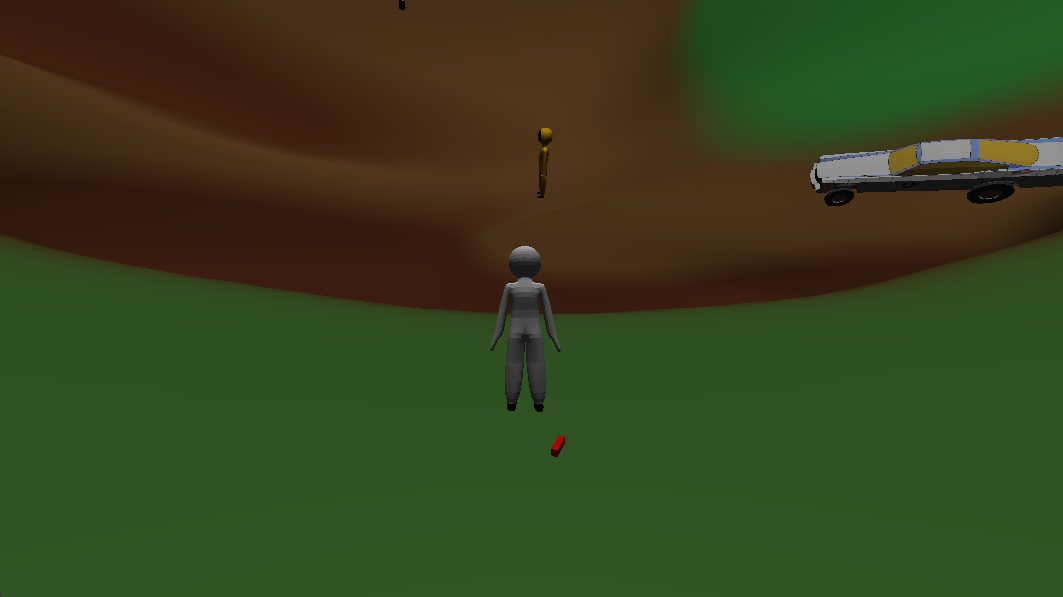
\includegraphics[width=\textwidth]{chapters/problems/resources/just-before.png}
        \caption[]%
        {{\small Just before teleporation}}
        \label{fig:before-teleport}
    \end{subfigure}
    \hfill
    \begin{subfigure}[b]{0.475\textwidth}
        \centering
        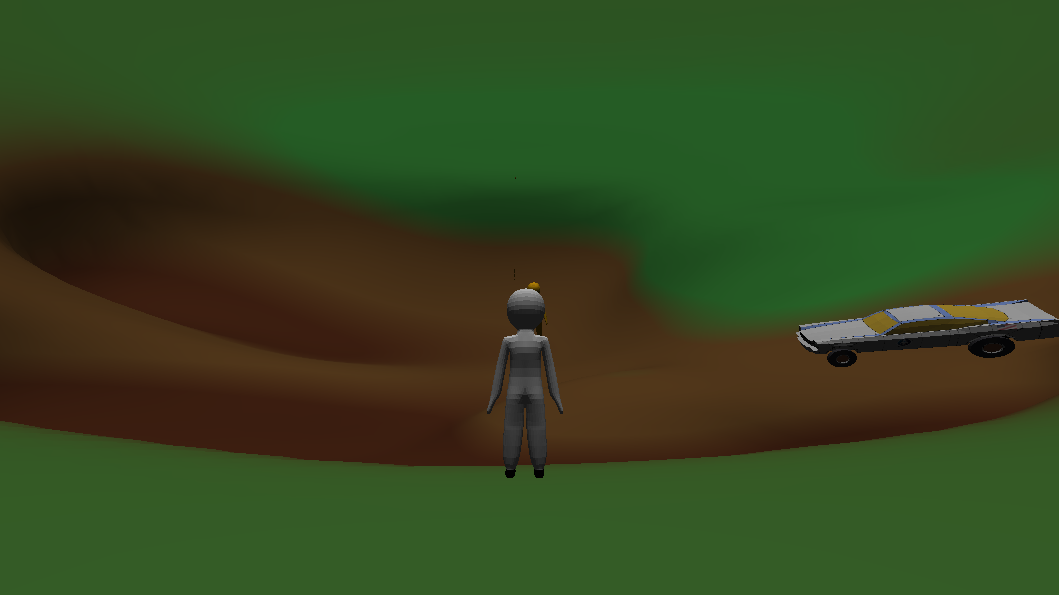
\includegraphics[width=\textwidth]{chapters/problems/resources/just-after.png}
        \caption[]%
        {{\small Just after teleportation}}
        \label{fig:after-teleport}
    \end{subfigure}
    \caption[]
    {\small Camera jump resulting from teleporation}
    \label{fig:camera-jump-teleport}
\end{figure}